\documentclass[output=paper]{langsci/langscibook} 
\author{Hansjakob Schneider\affiliation{Zurich University of Teacher Education}\orcid{}}
\title[Language aptitude in German and English in primary school]
      {Language aptitude in German as a school language and English as a foreign language in primary school}
\abstract{Two cases of language learning (English as a foreign language and German as the language of instruction) were compared using data from the LAPS II project. Hierarchical Regression Analyses were performed with achievement in English or German respectively as dependent and language aptitude components as well as other cognitive and language-related variables as independent variables. Results suggest that language aptitude variables are strong predictors of achievement in English as a foreign language and to a lesser degree for German as the language of schooling. Language self-concepts play an important role in achievement in English and less so in German. In the case of German (but not of English), socioeconomic status is a strong predictor of achievement Since these analyses were exploratory, further research is needed to come to conclusions relevant for language teaching.}
\IfFileExists{../localcommands.tex}{
  \addbibresource{localbibliography.bib}
  % add all extra packages you need to load to this file

\usepackage{tabularx,multicol}
\usepackage{url}
\urlstyle{same}

\usepackage{listings}
\lstset{basicstyle=\ttfamily,tabsize=2,breaklines=true}

%\usepackage{langsci-optional}
\usepackage{langsci-lgr}
\usepackage{langsci-gb4e}
\usepackage{langsci-optional}

\usepackage{enumitem}
\usepackage[group-digits=false, detect-weight=true]{siunitx}

\usepackage{todonotes}

  \newcommand*{\orcid}{}
 
  %% hyphenation points for line breaks
%% Normally, automatic hyphenation in LaTeX is very good
%% If a word is mis-hyphenated, add it to this file
%%
%% add information to TeX file before \begin{document} with:
%% %% hyphenation points for line breaks
%% Normally, automatic hyphenation in LaTeX is very good
%% If a word is mis-hyphenated, add it to this file
%%
%% add information to TeX file before \begin{document} with:
%% %% hyphenation points for line breaks
%% Normally, automatic hyphenation in LaTeX is very good
%% If a word is mis-hyphenated, add it to this file
%%
%% add information to TeX file before \begin{document} with:
%% \include{localhyphenation}
\hyphenation{
affri-ca-te
affri-ca-tes 
Soa-res
scru-ti-ny
me-ta-cog-ni-tion
}

\hyphenation{
affri-ca-te
affri-ca-tes 
Soa-res
scru-ti-ny
me-ta-cog-ni-tion
}

\hyphenation{
affri-ca-te
affri-ca-tes 
Soa-res
scru-ti-ny
me-ta-cog-ni-tion
}
 
  \togglepaper[1]%%chapternumber
}{}

\begin{document}
\SetupAffiliations{mark style=none}
\maketitle 
%\shorttitlerunninghead{}%%use this for an abridged title in the page headers


\section{Introduction}

In the previous chapters the focus has been on English or French as foreign languages. Language aptitude is indeed a concept which in research is more often linked with foreign language learning rather than untutored second language acquisition or first language acquisition (untutored in early childhood or tutored in school). The present chapter explores the relationship between language aptitude and achievement in German as a school language (GSCL) and compares it to the case of English as a Foreign Language (EFL).

The objective of this chapter is to find out if achievement in EFL and in GSCL share common influencing factors and to identify them. The role of aptitude in language learning and its position in the field of potentially influential other factors is of particular interest. In this respect the quantitative-analytical procedure employed is exploratory. 

In \sectref{sec:09:2} theoretical and empirical findings about the role of language learning aptitude are discussed. The study design is presented in \sectref{sec:09:3.} \sectref{sec:09:4} contains statistical analyses: Results on the achievement in EFL and GSCL are presented and variables with a high influence on the achievement in these languages are identified. 

The results are discussed in \sectref{sec:09:5} in view of the theory of language aptitude.

The analyses used are similar to the ones in Chapter 4 and yet different in specific ways. The main focus of the research presented in this volume is on foreign language learning and the data we collected pertains mainly to this matter. This includes ID variables beyond aptitude for EFL (e.g. different kinds of motivation). In Chapters 3 and 4, EFL was conceptualized as the dependent variable, while achievement in GSCL was designed to be one of the independent variables. Since EFL had a special status in the LAPS II study, some language-specific data were collected for EFL only and not for German. Therefore, the choice of variables to be compared was restricted to variables not specific to either language (working memory for instance) and to self-concept (which was collected for English as well as for German). For a full account of the situation for EFL see Chapters 3 and 4.

\section{Aptitude and related variables in EFL- and GSCL-learning}

For foreign language learning in school there is plenty of evidence that aptitude has significant impact on the learning outcome \citep{Li2015}. Studies which investigate language aptitude in the acquisition of first languages and especially in learning first languages as the languages of schooling on the other hand are rather scarce (but see e.g. \citealt{SkehanDucroquet1988}). Generally the impact of aptitude on learning the language of instruction in school is less easily proven, maybe because the “massive exposure time and experience with native languages overrides genetic influences and ‘levels them out' – influences and differences which would potentially have been there in the first place as well.” (\citealt{Reiterer2018}: ix)

Learning the language used in the general school-context (language of instruction) is an interesting case of language acquisition and learning: On the one hand, it relies heavily on first language acquisition (at least in situations where it is identical or related to the first language of the areas in question). On the other hand, in school the basic skills of reading and writing are introduced and fostered; moreover, with the \textit{language of schooling} \citep{Schleppegrell2004} features of language which can be quite different from everyday language use come into play. The few existing studies about untutored vs. tutored L2 learning/acquiring present contradictory results as far as the role of language learning aptitude is concerned (\citealt{UdryEtAl2019}).\footnote{No studies comparing the influence of language aptitude in the cases of untutored acquisition vs. learning of L1 at school are known to me.} In Li’s meta-analysis of research on associations between aptitude and grammar learning, aptitude showed significant effect sizes also in non-tutored contexts; however, Li views these results critically because the studies reviewed lack control over the acquisition contexts of the participants \citep[405]{Li2015}. There is, however, empirical support for the thesis that language learning aptitude plays a role not only in foreign language learning/acquisition but also in first language acquisition (\citealt{BiedronPawlak2016}).

Beyond language learning aptitude there is a number of variables which have proved to contribute significantly to L2- and L1-learning (for a detailed account see Chapter 1). For the purposes of this chapter I will present only the ones for which data were collected for both EFL and GSCL (for detailed information see Chapter 1).

Nonverbal fluid intelligence is related closely to learning in general, to language aptitude and hence to L2 learning as well (see Chapter 1); it does correlate with aptitude, but can be differentiated from it (\citealt{SparksEtAl2012}). Fluid intelligence is also a moderate predictor of school-related abilities in L1 (such as reading comprehension, \citealt{PengEtAl2019}).

Another nonlinguistic variable is working memory. Working memory, like nonverbal intelligence, is a concept with impact on many forms of learning. Its influence on L2 learning in the context of aptitude studies has been empirically proven (\citealt{WenEtAl2017}, see also Chapter 1). Working memory also influences L1 reading comprehension at school (e.g. \citealt{PengEtAl2017}).

Competence in L1 has been recognized in recent years as an important variable for foreign language learning. Sparks and his colleagues have put forward their linguistic coding difference hypothesis (LCDH) and have gathered sound empirical evidence to show that attainment in L1 predicts learning outcomes in L2 on secondary school level (\citealt{SparksEtAl2012}; \citealt{Li2016}).

In a similar vein, in a longitudinal study (grades 1-10) \citet{SparksEtAl2012} determined the effect sizes of L2 aptitude, L1 skills, IQ and other variables on various facets of L2 proficiency using Hierarchical Regression Analyses. They found strong influences of a composite of L1 skills, IQ and aptitude on all areas of L2 proficiency; in the case of reading comprehension in L2 the variance accounted for by this composite was 45\%. Unfortunately, the unique roles of aptitude and IQ were not reported separately. 

The role of language self-concept in L2-learning is reported in Chapters 1, 3, 4 and 8. As for reading comprehension in GSCL there is evidence from a large longitudinal study for the skill-development hypothesis (achievement predicts self-concept) as well as for reciprocal effects (in addition to skill-development hypothesis: self-concept predicts achievement, especially around grade 5, \citealt{RetelsdorfEtAl2014}).

The impact of socio-economic status (SES) on school achievement in general is well documented (see the meta-analysis by \citealt{Sirin2005}). For its influence on EFL in the LAPS project see Chapter 5. Its status for reading comprehension in GSCL is undisputed: A vast number of empirical studies have proven a strong influence of SES on reading comprehension in school contexts for all grades \citep{Schaffner2009}.

The conclusion of all these findings is that both for EFL and GSCL learning is a multivariate process. But is the influence of aptitude (in the context of the above-mentioned variables) on learning EFL similar to learning GSCL? In other words: Do aptitude variables influence tutored L1- and L2-learning in a similar way or is there a difference in strength (effect size) and kind of aptitude components (e.g. grammatical sensitivity vs. inductive ability)? From these questions the following objective can formulated:

The main objective of the current article is quantify the effect of language aptitude on GSCL in comparison to EFL. 

\section{Study design and method}

The data to be analysed here stem from the LAPS II study. Since the general design of the study is described in Chapter 2 I will only go into aspects of the design which are specific to the research objective mentioned at the end of the last section. 

The data come from the LAPS II sample ($n(\text{T2})=578$, $n\text{(T3)}= 566$, cf. Chapter 2.4.1.5). The sample size in this chapter is not identical because only students were included for whom data for the two measurement points and for all variables in question were available. For this reason, the number of participants varies depending on the type of analysis carried out. Furthermore, outliers and students with English as L1 were excluded.

In the following the two age groups, 1 (grade 4 to 5) and 2 (grade 5 to 6), are treated separately for reasons to be presented in \sectref{sec:09:4.}

Whereas Chapters 3 and 4 in this volume are concerned with understanding the underlying dimensions of EFL (Chapter 3) and predicting achievement in EFL (Chapters 4 and 5), a different approach is taken in the present chapter: The main idea of the following analyses is to compare the influence of language aptitude on performance in EFL and GSCL respectively, taking into account variables collected for both languages. On the one hand, these are variables of nonlinguistic nature (e.g. general cognitive variables, Socioeconomic Status), on the other hand, (cognitive-linguistic) aptitude variables. Furthermore, the respective self-concepts for EFL and GSCL are also included in the analyses.

Excluded are all variables which are not available for both languages. These are mainly the variables of language learning motivation (only available for English). It seems obvious that a comparison of influencing variables in EFL and GSCL should draw on the same or similar variables. As mentioned in the introduction, the consequence of this procedure is that the results cannot be compared to similar analyses of EFL alone in Chapters 3 and 4.

Hierarchical regression models were fitted to the data to identify the variables that predict performance in English and German. The following variables were included in the analyses, achievement in English and German being the dependent variables (For a more detailed description see Chapter 2):

\begin{description}
\item[Achievement in English as a foreign language (EFL):]
This variable was measured using the Oxford Young Learners Proficiency Test (OYLPT) for T1 and a c-test for T2 and T3. Since the OYLPT does not measure the same linguistic dimensions as the c-tests (it includes a listening comprehension part, for instance) only measurement point T3 will be included in the analysis of predicting variables (cf. \sectref{sec:09:4.2} for further details). C-tests have proved to be a valid measure for general language proficiency (\citealt{EckesGrotjahn2006}).
\item[Achievement in German as the school language (GSCL):]
For all three measurement points the sentence reading part of the ELFE test (\citealt{LenhardSchneider2006}) was administered. ELFE is a widely used standardised test covering grades 1 to 6. Within narrow time limits students are confronted with a series of incomplete sentences. In each sentence they must choose one of 5 words to form a correct sentence; a translated example would be:\\
Lea is playing (after / next to / \textbf{instead} / then / that) of learning. \\
The test addresses primarily the dimensions of vocabulary and of grammar. In this sense it covers similar dimensions as the c-tests used for measuring achievement in EFL (but not the productive component of coming up with a suitable word). The measure was the number of sentences completed correctly per minute.
\item[Grammatical sensitivity (MLAT, Part 2):]
This test is a translated and adapted version of the MLAT-E, Part 2 (\citealt{CarrollSapon2010}). 
\item[Inductive ability (PLAB):]
For inductive ability a translated and adapted version of part 4 of the PLAB (\citealt{PimsleurEtAl2004}) was used.
\item[Phonemic coding ability (Llama):]
We used Llama-D, the phonemic discrimination task in which students had to recognize sounds (\citealt{MearaEtAl2001}).
\item[Verbal working memory (backwards digit span):]
Verbal working memory was tested with a task in which students had to memorize a sequence of numbers (increasing in length) in backward order.
\item[Visuospatial working memory (Corsi block task):]
Visuospatial working memory was tested using an adaptation of the Corsi block task. Students had to remember the order of an increasing number of squares lit up from a matrix of squares.
\item[Field independence (group embedded figures test):]
Participants had to find simple geometrical figures embedded in more complex figures under time pressure \citep{OltmanEtAl1971}.
\item[Fluid intelligence (CFT):]
Students had to discover rules for example in comparing sequences of increasingly complex matrices \citep{Weiss2006}.
\item[Socioeconomic status, economic and cultural aspects (SES):]
In line with the theoretical assumptions and empirical findings in Chapter 5, the construct of the SES is split up into two dimensions: economic and cultural aspects (for the variables involved in each dimension see Chapter 5).
\end{description}

The data was statistically analysed using SPSS (version 27 for Macintosh). Procedures included repeated measurement ANOVAS (used to determine whether the two age groups behave similarly) as well as hierarchical stepwise regression analyses (used to establish the kind and strength of influencing variables).

\section{Results}
\subsection{ Achievement in German as a School Language and English as a foreign language} %4.1 /

Since the sample of the longitudinal LAPS II study consisted of two age groups (grades 4 to 5; grades 5 to 6) it had to be established first if the development in achievement of English (and of German) was homogeneous for the two groups. As shown in Chapter 4 the variable age group (grade 4 or 5 respectively at T1) contributes to attainment in English at T3. There seems to be good reason to assume that the two age groups behave differently as far as learning EFL and other variables mentioned are concerned. To get a more detailed view of the role the two age groups play, a repeated measures variance analysis with the three measurements of English (\figref{fig:09:1}) and of German (\figref{fig:09:2}) as dependent and the age group (1 and 2) as the independent variables was performed. Figures 1 and 2 show that the (younger) age group 1 develops more positively than age group 2. 

Z-standardized values were used to make the effects more visible. In \figref{fig:09:1} age group 1 not surprisingly has relatively lower mean measures for achievement in EFL than age group 2 (students of age group 2 having profited of one more year of English lessons). Z-transformed values can be negative (as is the case for all means of age group 1). This means that they are below average of the whole sample (the average of the whole sample being standardized at the value 0). 

 \begin{figure}
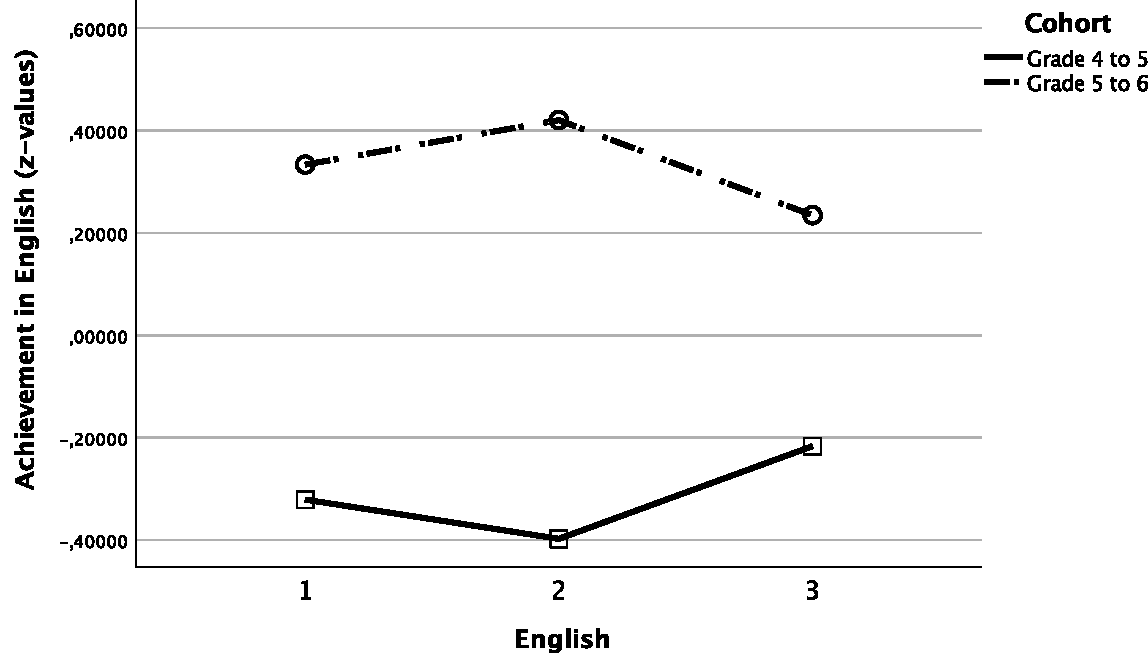
\includegraphics[width=\textwidth]{figures/figure9.1.pdf}
\caption{The development of test results in English (standardized) from T1 to T3 for the two age groups (grades 4 to 5, grades 5 to 6); Repeated Measures ANOVA: within subjects (measurements T1–T3)*between subject (age groups) effects significant (Greenhouse-Geisser, $F=14.37$, $\text{df}=1.65$, $p<0.001$); covariates: fluid intelligence CFT 20 ($F=45, p<0.001$); SES ($F=13.44, \text{df}=1, p<0.001$)}
\end{figure}

\begin{figure}
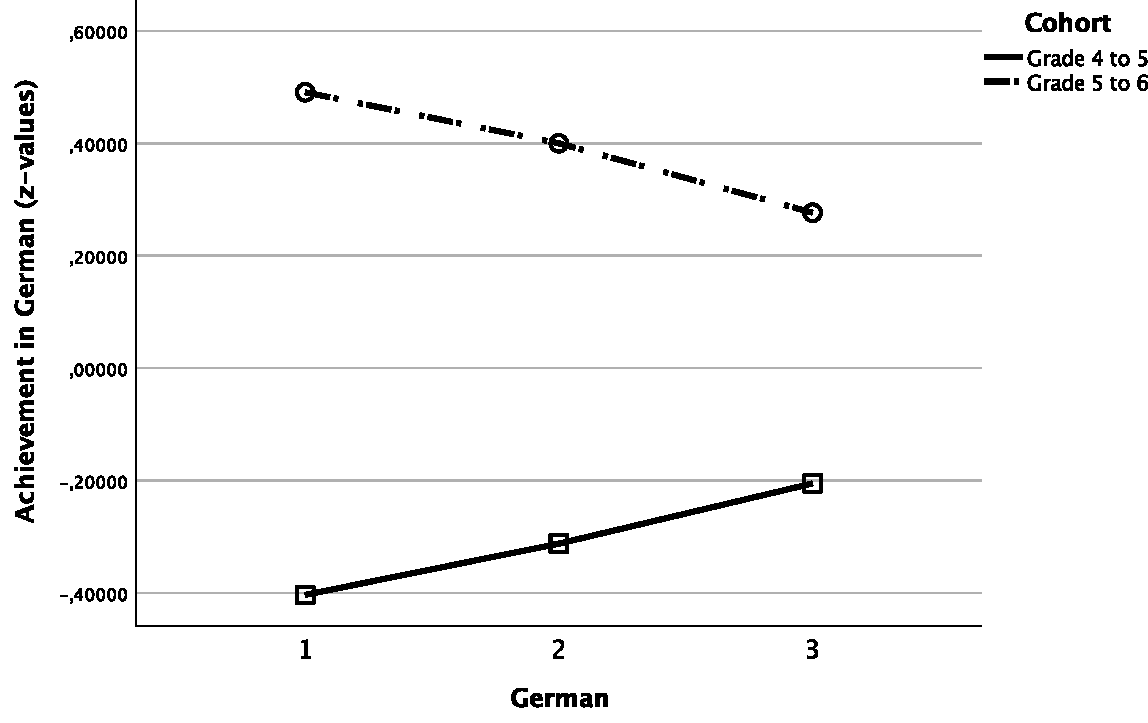
\includegraphics[width=\textwidth]{figures/figure9.2.pdf}
\caption{The development of test results in German (standardized measures of the ELFE-subtest on sentence reading) T1 to T3 for the two age groups (grades 4 to 5, grades 5 to 6); Repeated Measures ANOVA: within subjects (measurements T1–T3)*between subject (age groups) effects significant (Greenhouse-Geisser, $F=22.53, \text{df}=1.94, p<0.001$); covariates: fluid intelligence CFT 20 ($F=64.86, p<0.001$); SES ($F=52.76, \text{df}=1, p<0.001$)}
\end{figure}

In both EFL and GSCL the difference in achievement between the two age groups diminishes with time. This means that towards the end of primary school (between grades 5 and 6) learning in EFL as well as in GSCL slows down whereas between grade 4 and 5 (age group 1, T1–T3) more learning takes place. The repeated measures ANOVAs reported in Fig. 1 and 2 prove that the interaction between the age groups and the development of achievement in either language is significant, i.e. that the two groups develop differently in English and in German.

These results led to the decision to perform further analyses separately for the two age groups.

Another element which links the development of EFL and GSCL is stability over time: although obviously the students’ test results increase over the period of almost two years, they are highly correlated for the three measurement points. Tables 1 and 2 show the Pearson correlations of the test results for the English and the German test respectively.

\begin{table}
\sisetup{table-space-text-post = {***}}
\begin{tabular}{l *{6}{S[table-format=1.2,table-align-text-post=false]}} 
\lsptoprule
& \multicolumn{3}{c}{Age group 1} & \multicolumn{3}{c}{Age group 2}\\\cmidrule(lr){2-4}\cmidrule(lr){5-7}
     & {E T1} & {E T2} & {E T3} & {E T1} & {E T2} & {E T3}\\\midrule
E T1 & 1 & 0.67*** & 0.65*** & 1 & 0.72*** & 0.71***\\
E T2 &   & 1      & 0.84*** &   & 1      & 0.88***\\
E T3 &   &        & 1      &   &        & 1\\
\lspbottomrule
\end{tabular}
\caption{Pearson correlations of test results in English for age groups 1 and 2 from T1 to T3; ***: $p<0.001$,  agegroup 1 $n= 252$, age group 2 $n=286$.}
\end{table}

\begin{table}
\sisetup{table-space-text-post = {***}}
\begin{tabular}{l *{6}{S[table-format=1.2,table-align-text-post=false]}} 
\lsptoprule
& \multicolumn{3}{c}{Age group 1} & \multicolumn{3}{c}{Age group 2}\\\cmidrule(lr){2-4}\cmidrule(lr){5-7}
     & {G T1} & {G T2} & {G T3} & {G T1} & {G T2} & {G T3}\\\midrule
G T1 & 1    & 0.79*** & 0.74*** & 1 & 0.80*** & 0.77***\\
G T2 &      & 1       & 0.76*** &   & 1 & 0.75***\\
G T3 &      &         & 1 &     &   & 1\\
\lspbottomrule
\end{tabular}
\caption{Pearson correlations of test results in German for age groups 1and 2 from T1 to T3; ***: $p<0.001$, agegroup 1 $n= 260$, age group 2 $n=283$.}
\end{table}

The test results are so strongly correlated that the assumption of common underlying factors (one for the three English measures and one for the three German measures) lends itself. Similarly, both aptitude variables used in our study (grammatical sensitivity and inductive ability) are shown in Chapter 10 to be remarkably stable over time.

In the next section the impact of language aptitude on achievement in English and in German is analysed.

\subsection{Influencing variables on German as a school language and English as a foreign language} %4.2 /

One of the interesting questions in the theory of language aptitude pertains to the specificity of the aptitude concept for foreign language learning, second language acquisition, first language acquisition and school language learning. Of these four different situations the LAPS II project is able to compare foreign language learning with school language learning (which is partly connected to first language acquisition in that it builds upon the latter but introduces novel dimensions like reading or writing, see \sectref{sec:09:2}). The variables included in the statistical model can be grouped into three sections:

\begin{enumerate}
\item Language-learning specific
   \begin{enumerate}[label=\alph*.]
   \item Grammatical sensitivity (MLAT)
   \item Inductive ability (PLAB)
   \item Phonemic encoding (Llama)
   \item Self-concept for English/German
   \end{enumerate}
\item General cognitive
   \begin{enumerate}[label=\alph*.]
   \item Working memory (Backward digit span, Corsi blocks)
   \item Field independence (GEFT)
   \item Nonverbal fluid intelligence (CFT)
   \end{enumerate}
\item Sociodemographic
   \begin{enumerate}[label=\alph*.]
   \item Socio-economic status (economic)
   \item Socio-economic status (cultural)
   \end{enumerate}
\end{enumerate}

The following analyses use multiple stepwise regression analyses to establish the nature and effect size of influencing variables on the achievement in English and in German. The aim is to compare the patterns found for achievement in English and in German. In contrast to Chapter 4 the achievement measures of the two languages at T1 are not included as predictors of T3 for the following reason: The English test at T1 (OYLPT) is not the same as at T3 (c-test), whereas for German it is (ELFE). A comparison of the patterns of influencing variables for the two languages would be affected by this inequality. 

In comparing the predicting variables for achievement in English and in German the respective measures for T3 (i.e. English c-test T3 and ELFE test T3) were chosen as the dependent variables. Of the language-learning-specific variables mentioned above the measures for T1 were entered into the analyses as predictors for the T3 outcome variables. Since the nature of these analyses is exploratory the stepwise method is applied, which means that the independent variables selected in the model are chosen not for theoretical reasons but purely for their ability to contribute significantly to explaining variance \citep[213]{Field2009}. The strongest variable is chosen first, the second variable is the one which explains most of the remaining variance and so forth. All variables mentioned above were included in the models but only the variables leading to significant changes in explained variance (R\textsuperscript{2})\textsuperscript{} are reported in the tables. Tables 3 and 4 show the results of these analyses for EFL (age groups 1 and 2 respectively).

\begin{table}
\sisetup{table-space-text-post = {***}}
\fittable{\begin{tabular}{l ccc S[table-format=2.2,table-align-text-post=false]}
\lsptoprule
& R\textsuperscript{2} & Corrected R\textsuperscript{2} & Change in R\textsuperscript{2} & {Change in F}\\\midrule
\textit{Model 1}: SCE T1 & 0.23 & 0.23 & 0.23 & 51.00***\\
\textit{Model 2}: Model 1 + IA T1 & 0.33 & 0.32 & 0.10 & 23.91***\\
\textit{Model 3}: Model 2 + FI T1 & 0.37 & 0.36 & 0.04 & 10.91**\\
\textit{Model 4}: Model 3 + BDS T1 & 0.40 & 0.38 & 0.03 & 6.68*\\
\textit{Model 5}: Model 4 + PCA T1 & 0.41 & 0.39 & 0.02 & 4.10*\\
\lspbottomrule
\end{tabular}}
\caption{Grade 5 – results of the stepwise multiple regression analysis for achievement in English (c-test T3) with predictors T1, ***: $p<0.001$, **: $p<0.01$, *: $p<0.05$; $n=170$. SCE: Self-concept English, IA: Inductive ability, FI: Fluid intelligence, BDS: Backward digit span, PCA: Phonemic coding ability}
\end{table}

\begin{table}
\sisetup{table-space-text-post = {***}}
\fittable{\begin{tabular}{l ccc S[table-format=2.2,table-align-text-post=false]}
\lsptoprule
& R\textsuperscript{2} & Corrected R\textsuperscript{2} & Change in R\textsuperscript{2} & {Change in F}\\\midrule
\textit{Model 1}: GS T1 & 0.26 & 0.26 & 0.26 & 78.59***\\
\textit{Model 2}: Model 1 + SCE T1 & 0.39 & 0.38 & 0.12 & 44.05***\\
\textit{Model 3}: Model 2 + IA T1 & 0.42 & 0.42 & 0.04 & 14.26***\\
\lspbottomrule
\end{tabular}}
\caption{Grade 6 – results of the stepwise multiple regression analysis for achievement in English (c-test T3) with predictors T1; $***p<0.001$; $n= 223$. GS: Grammatical sensitivity, SCE: Self-concept English, IA: Inductive ability.}
\end{table}

The models for the two age groups are similar in the sense that their strongest predictor variables are comparable: self-concept English and components of aptitude. In the final model of grade 5, general fluid intelligence and verbal working memory have minor influence as well. Interestingly, fluid intelligence, a strong predictor of achievement at school in general, seems to lose some of its predictive power to the more language specific language aptitude variables. The variables that turn out to be most predictive in these models belong to the ones that have been shown to be positively associated with foreign language achievement in Chapters 3 and 4.

The models of the two age groups for achievement in German (cf. Tables 5 and 6) are also similar in that the respective final models include the same predictors: language aptitude (grammatical sensitivity), self-concept German, and SES (cultural aspects). Fluid intelligence, the strongest predictor for younger students (grade 5) does not show a significant effect in the older age group (grade 6). For the older students grammatical sensitivity is the leading predictor of achievement in German.

\begin{table}
\fittable{\begin{tabular}{l ccc S[table-format=2.2,table-align-text-post=false]}
\lsptoprule
        & R\textsuperscript{2} & Corrected R\textsuperscript{2} & Change in R\textsuperscript{2} & {Change in F}\\\midrule
\textit{Model 1}: FI T1 & 0.16 & 0.16 & 0.16 & 32.54***\\
\textit{Model 2}: Model 1 + SESc T1 & 0.23 & 0.23 & 0.07 & 15.74***\\
\textit{Model 3}: Model 2 + SCG T1 & 0.27 & 0.26 & 0.03 & 7.79**\\
\textit{Model 4}: Model 3 + GS T1 & 0.29 & 0.27 & 0.02 & 4.60*\\
\lspbottomrule
\end{tabular}}
\caption{Grade 5 – results of the stepwise multiple regression model for achievement in German (ELFE T3) and predictors T1; *** $p<0.001$, ** $p<0.01$, $n=170$. FI: Fluid intelligence, SESc: SES (cultural), SCG: Self-concept German, GS: Grammatical sensitivity.}
\end{table}

\begin{table}
\fittable{\begin{tabular}{l ccc S[table-format=2.2,table-align-text-post=false]}
\lsptoprule
& R\textsuperscript{2} & Corrected R\textsuperscript{2} & Change in R\textsuperscript{2} & {Change in F}\\\midrule
\textit{Model 1}: GS T1 & 0.17 & 0.16 & 0.17 & 43.33***\\
\textit{Model 2}: Model 1 + SESc T1 & 0.21 & 0.20 & 0.04 & 11.24**\\
\textit{Model 3}: Model 2 + SCG T1 & 0.23 & 0.22 & 0.02 & 5.63*\\
\lspbottomrule
\end{tabular}}
\caption{Grade 6 – results of the stepwise multiple regression model for achievement in German (ELFE T3) and predictors T1; *** $p<0.001$, ** $p<0.01$, * $p<0.05$, $n=222$}
\end{table}

In conclusion we can state that for English and also for German (and for both age groups) aptitude variables (inductive ability, grammatical sensitivity, and phonemic coding ability in English; grammatical sensitivity in German) play a key role in accounting for achievement. They explain more unique variance for EFL (12\% and 30\%) than for GSCL (between 2 and 17\%). SES seems to be more important in learning GSCL than EFL. Moreover, general fluid (nonverbal) intelligence accounts for variance in the models for the younger students but not for the older ones. It seems that nonverbal intelligence is replaced as a predictor by the more language specific aptitude measures. Finally, language self-concept is a relatively stronger predictor for achievement in EFL than in GSCL.

\section{Discussion}

The main objective of the present chapter was to quantify the effect of language aptitude on EFL and GSCL. The short conclusion is this: Of all the language-learning specific, general cognitive and sociodemographic measures, language learning aptitude (mainly in the facets of grammatical sensitivity and inductive ability) and self-concept overrule the other variables in the case of achievement in English. For German the influence of language aptitude variables is weaker and it differs between the two age groups. In the case of EFL the strongest aptitude variable for the younger students is inductive ability, for the older students grammatical sensitivity takes the lead. In the case of GSCL grammatical sensitivity is the strongest aptitude variable for both age groups.

The more detailed conclusion focuses on two aspects: (a) The stability over time of some of the constructs presented, (b) structural differences between learning EFL vs. GSCL. 

(a) The high correlations between the achievement measures in English and German over the period from grades 4 to 6 suggests that while achievement increases during this period (i.e. the students improve intra-individually) there seems to be one underlying ability for EFL and one for GSCL (there isn’t much inter-individual variation in either language, high and low achievers for example remain high and low over time) In the same sense but to a slightly lesser degree grammatical sensitivity and inductive ability are stable over time (cf. Chapter 10).

(b) The structure and strength of the influencing variables was shown to be very similar for the achievement in English and the achievement in German. The aptitude variables \textit{grammatical sensitivity} and \textit{inductive ability} explain a large part of the variance in the regression models for EFL. This strong influence of language aptitude variables on foreign language learning is well documented (e. g \citealt{Li2016}) and not surprising. 

The lower influence of language aptitude (in the form of grammatical sensitivity) on the comprehension of German sentences (Tables 5 and 6) may be attributed to differing situations of acquisition: In grades 4 to 6 the predominant part of students has reached an achievement level in German which exceeds their achievement in English by far. As discussed in \sectref{sec:09:2} the influences of language aptitude may have been levelled out by vast experience with the language.

Whereas in EFL inductive ability is a predictor for achievement (especially for the younger age group), in the case of GSCL it doesn’t seem to play a much weaker part (relative to grammatical sensitivity). This fact could be interpreted along the following lines: In the case of German (as L1) the period of having to induce grammatical rules and structures is long past for most students: They don’t have to induce grammatical rules because they acquired them in earlier stages (mostly in pre-school acquisition). In contrast, the ability to recognise grammatical functions is an important prerequisite for selecting the correct alternative word in the sentences of the ELFE-test (is the word in the role of an agent, patient, theme etc.?). Therefore, grammatical sensitivity is a key feature in the context of this test.

In the case of English, the same reasoning holds true: To fill the gaps in the c-tests the function of the words in the sentence must be clear (and in addition morphosyntactic knowledge must be retrieved). Why in age group 1 (grade 4 to 5) inductive ability is a stronger predictor than grammatical sensitivity is difficult to answer. Rule induction might be more important in the early stages of learning a language than in later stages.

Socioeconomic status significantly influences the achievement in German but not in English. This is probably attributable to the abundance of socially embedded experiences with the German language that speakers of German have made up to the age of 10 to 12. In the case of English, direct influence of family background is much shorter (English having only been taught for 2 to 3 years in our sample) and much less intensive (English is not generally spoken in families with German as L1). 

Results not reaching statistical significance may be at least as instructive as the statistically significant results discussed so far:\\
One aptitude variable, phonemic coding ability, proved to have only a marginal effect in our study. This can be explained by the nature of the language tests administered. Both for English and for German written texts (or sentences) were used. It could be argued that in reading as well as in listening phonemic coding plays a role. However, in reading the role of phonemic coding is especially important in the early stages of literacy development when students translate each grapheme into a phoneme and store it in a buffer until the whole word has been synthesized. According to the dual coding theory (cf. \citealt{ColtheartEtAl2001}) another cognitive path becomes more and more dominant as proficiency in reading increases: it leads from orthographic analysis (a graphemic representation of a word) directly to the orthographic lexicon, and from there to the semantic system; the semantic content is then matched to the corresponding phonemic representation as a whole (i.e. without analysing or synthesizing). The role of phonemic coding ability in this route is minimal and therefore the Llama test accounts for hardly any variance in the reading of English or German (though more in early stage EFL than in advanced GSCL). Its position might have been quite different had the tests involved speaking or listening activities. The same goes for verbal working memory: Had the tests involved oral language, verbal working memory might have played a more important role. 

The relatedness of intelligence and language aptitude has been discussed in the literature (and empirically proved in Chapter 3) and the upshot is that they are closely related but distinguishable constructs (e.g. \citealt{Li2016}: 826f.). When using stepwise multiple regression models this situation may lead to one of two closely competing variables to take the lead (and explain most of the unique variance) leaving its competitor with only a small part of explained variance. This seems to be the case for sentence comprehension in German: For students in grade 5 fluid intelligence is the strongest predictor (\tabref{tab:09:5}) whereas for the sixth formers grammatical sensitivity takes the lead.

Two final words of caution: Firstly, the tests used for measuring achievement in English (c-tests) and German (sentence comprehension) are similar but not identical (c-tests require productive skills to a higher degree). Some of the differences in the patterns of influencing variables may be attributable to these differences. However, since according to Li’s meta-analysis on the influence of language aptitude on language learning the language analytic component is relatively weakly correlated with the productive skills of speaking and writing (\citealt{Li2016}: 823f.), the difference between the tests may not be all that important for the pattern of grammatical sensitivity and inductive ability in the English and German models.

Secondly, the analyses performed for the purposes of this chapter are exploratory in nature. While they do show the trend for language aptitude variables to be the strongest predictors for achievement in EFL and have some influence in GSCL, it would be too early to draw specific conclusions for teaching at school. Rather, further research should investigate whether aptitude variables can be effectively taught in school settings and what their impact is on various measures of achievement (grammar, listening, reading, speaking, and writing).
\sloppy\printbibliography[heading=subbibliography,notkeyword=this]
\end{document}
